
\documentclass[10pt,a4paper]{article}
\usepackage[top=0.85in,left=1in,footskip=0.75in]{geometry}
% amsmath and amssymb packages, useful for mathematical formulas and symbols
\usepackage{amsmath,amssymb}

\usepackage{changepage}
% Use Unicode characters when possible
\usepackage[utf8x]{inputenc}
% textcomp package and marvosym package for additional characters
\usepackage{textcomp,marvosym}
% cite package, to clean up citations in the main text. Do not remove.
\usepackage[superscript,biblabel]{cite}
% Use nameref to cite supporting information files (see Supporting Information section for more info)
\usepackage{nameref,url}
% line numbers
%\usepackage[right]{lineno}


% color can be used to apply background shading to table cells only
\usepackage[table]{xcolor}

% array package and thick rules for tables
\usepackage{array}

\usepackage{dsfont}

\usepackage{graphicx}

\usepackage{todonotes}

%% END MACROS SECTION

\title{Prosit Transformer: A transformer for prediction of MS2 spectrum intensities}
\author{Markus Ekvall$^1$ \and Patrick Truong$^1$ \and Wassim Gabriel$^2$ \and Mathias Wilhelm$^2$ \and Lukas K\"{a}ll$^1,^*$}
\date{}

\begin{document}
%\linenumbers
\maketitle
$^1$Science for Life Laboratory, School of Engineering Sciences in Chemistry, Biotechnology and Health, Royal Institute of Technology -- KTH, Box 1031, SE-17121 Solna, Sweden\\
$^2$Computational Mass Spectrometry, Technical University of Munich (TUM), D-85354 Freising, Germany\\
$^*$ Corresponding author, \url{lukas.kall@scilifelab.se}

\begin{abstract}
Machine learning has been an integral part of interpreting data from mass spectrometry-based proteomics for a long time. Relatively recently, a machine-learning structure appeared successful in other areas of bioinformatics, Transformers. Furthermore, the implementation of Transformers within bioinformatics has become relatively convenient due to transfer learning, i.e., adapting a network trained for other tasks to new functionality. Transfer learning makes these relatively large networks more accessible since it generally requires less data, and the training time improves substantially.
We implemented a Transformer based on the pre-trained model TAPE to predict MS2 intensities. TAPE is a general model trained to predict missing residues from protein sequences. Despite being trained for a different task, we could modify its behavior by adding a prediction head at the end of the TAPE model and fine-tune it using the spectrum intensity from the training set to the well-known predictor Prosit.
We demonstrate that the predictor, which we call Prosit Transformer, outperforms the recurrent neural network-based predictor Prosit, increasing the median angular similarity on its hold-out set from 0.908 to 0.929.
We believe that transformers will significantly increase prediction accuracy for other types of predictions within mass spectrometry-based proteomics.
\end{abstract}

{\bf Keywords:} Machine Learning; Proteomics; MS2 spectra; Transformers

\section*{Introduction}
Just as in many other areas involving analysis of large and complex datasets, different types of machine learning are tremendously helpful for the modern analysis of mass spectrometry-based proteomics data \cite{Meyer2021-hc,Mann2021-kx}. For example, we nowadays can use machine learning to predict tryptic digestion \cite{Yang2021-ng}, chromatographic retention time \cite{Moruz2010-ls,Ma2018-wy,Martens_undated-vs}, collisional cross-section \cite{Meier2021-ur}, the accuracy of peptide-spectrum matches \cite{Kall2007-ll}, and the accuracy of transitions in DIA data \cite{Demichev2020-zd} are tasks that utilize machine learning.

One task that has gained traction in the last couple of years is predicting MS2 spectra from peptide sequences \cite{Degroeve2015-fh,Gessulat2019-el}. Such predictors can predict relative intensities of a given peptide sequence's $b$- and $y$-ions. Together with the m/z values of the ions, which one can derive from first principle, one can subsequently form a full MS2 spectrum. MS2 spectrum prediction has in a short time established itself as a means to rescore peptide spectrum matches \cite{C_Silva2019-ja}, increasing the sensitivity in large search spaces \cite{Wilhelm2021-mz}, and target-decoy strategies for DIA interpretation \cite{Searle2020-yk}.

Many types of frameworks are available for training a predictor, such as Support Vector Machines and Recurrent Neural Networks (RNNs) used within mass spectrometry-based proteomics. However, in the last couple of years, a structure first in natural language processing \cite{devlin2018bert} known as Transformers \cite{Vaswani2017-sy} has successfully been employed within bioinformatics, e.g., structure prediction \cite{Rao2019-qq,Bepler2021-ci}, gene expression prediction \cite{avsec2021effective}, and even within MS-based proteomics, e.g. peptide detection problem \cite{cheng2021pepformer}, DIA library generation for the phosphoproteome \cite{lou2021deepphospho} and {\em de novo} interpretation of MS2 spectra \cite{yilmaz2022novo}.

Transformers are, like RNNs, designed to handle sequential input data and do so through attention mechanisms, i.e., mechanisms that enhance the essential parts of the input sequence for its output. However, unlike RNNs, the Transformers do not use recurrence, thus enabling a significant speed-up by parallelizing their training. The encoder-decoder structure is the basis of the Transformers, where both the encoder and decoder adopt the multi-headed attention mechanism\cite{Vaswani2017-sy}.

Notably, the Tasks Assessing Protein Embeddings (TAPE) model \cite{Rao2019-qq} is exciting; a Transformer-based autoencoder of protein sequences is formed by withholding one amino acid at a time in a large set of protein sequences and subsequently predicting which is the missing amino acid. One can subsequently employ the model for higher-level tasks by plugging them into some extra layers of neurons in a process known as transfer learning \cite{Rao2019-qq,Bepler2021-ci}.

Here, we argue that Transformers can greatly aid mass spectrometry-based proteomics. We demonstrate that TAPE’s BERT sub-model, can predict MS2 spectrum intensities from peptide sequences. We are using the training and test sets of the popular Prosit \cite{Gessulat2019-el} predictor and demonstrate that the transformer-based predictor, which we named Prosit Transformer, drastically outperforms the old implementation of Prosit.

\section*{Methods}
\subsection*{Data}
We downloaded the Prosit training data from \url{https://figshare.com/projects/Prosit/35582}.  This set is composed of spectra from PXD004732, PXD010595, and PXD021013 \cite{Gessulat2019-el, Wilhelm2021-mz}. The Prosit data had to be converted from HDF5 to LMDB to be compatible with the Tape framework. The LMDB data files used during training and validation are accessible at \url{https://figshare.com/articles/dataset/LMDB_data_Tape_Input_Files/16688905}.

\subsection*{Architecture}

The TAPE model consists of twelve 768 hidden units attention layers, with the attention dropout (DropHead) rate \cite{Zhou2020-ji} and regular dropout rate set to 0.1. We downloaded weights for the pre-trained model that has been trained on the raw protein sequences in the protein families database (Pfam) to predict the amino acid at each protein position given the previous amino acids and the following amino acids \cite{Rao2019-qq}. The Prosit-specific transformer has the same parameter but consists of 9 attention layers. The meta-data layer is a multilayer perceptron (MLP) with two layers of size 512 units followed by a dropout rate of 0.1 each. The final prediction layer has the same structure, except for no dropout after the final layer.  The activation function is ReLU, except for the prediction layer where the first layer uses a ReLU6 \cite{Howard2017-yv}, i.e., a max(0,min(6,x)) function as an activation function, and the final layer uses a linear layer.

\subsection*{Metrics}

We measure angular distance, $d_{AB}=\frac{2}{\pi} \cos^{-1}\left(\frac{A \cdot B}{(||A||\cdot||B||)}\right)$, and angular similarity, $s_{AB} = 1 d_{AB}$ as measures of accuracy of the predicted intensities. Here, $A$ is the vector of predicted intensities, and $B$ is the vector of observed intensities for the ion series included in the prediction. However, we introduced a few extra steps during training to avoid undefined behavior. Firstly, to avoid undefined values using angular similarity during training, we had to clip the inputs to $\cos^{-1}$ with $-(1-\epsilon)$ and $(1-\epsilon)$ to avoid undefined values. This implementation was necessary since some predictions were too similar to their target after training, resulting in an undefined loss. However, there was no clipping during the evaluation, so it will not affect the final result. Lastly, we also had to introduce a small $\epsilon$ in the denominator in the cosine similarity, i.e., $\max(||A||\cdot||B||, \epsilon)$, to assure no undefined behavior during training. The sum of all $d_{AB}$ for all peptides in the test set was used as a loss function for the training of the networks. 

We calculated the $\mathit{FDR}=\mathit{FP}/(\mathit{FP}+\mathit{TP})$ and $\mathit{FNR}=\mathit{FN}/(\mathit{FN}+\mathit{TP})$ for each predicted spectrum to measure the number of erroneous peak predictions. Here $\mathit{FP}$ is the number of peaks predicted in excess to be present in a spectrum that was absent in the observed spectrum, $\mathit{FN}$ is the number of peaks deficently predicted to be absent in a spectrum that was present in the observed spectrum, and $\mathit{TP}$ is the number of peaks accurately predicted to be present in a spectrum that was present in the observed spectrum.

\subsection*{Post-processing of Predicted intensities}
We use the same post-processing on the predicted spectrum used in Prosit ​\cite{Gessulat2019-el} for the final result. To clarify, we set ions with a predicted negative intensity to zero, i.e., a negative intensity indicates an absent peak. Furthermore, we set all ion's intensity that's not obtainable for any given peptide due to too low a charge state or too low peptide length to -1. However, we exclude such peaks for similarity measurements. 

\subsection*{Hardware}

The model was trained on the Berzelius SuperPOD, a GPU cluster consisting of 60 NVIDIA DGX A100 systems, linked on a 200 Gbit/second NVIDIA Mellanox InfiniBand HDR network.

\section*{Results}
We set out to test whether Transformers are a technology fit for spectrum intensity predictions, i.e., to predict the intensities of the most commonly observed ion-series ($b^+, b^{2+}, b^{3+}, y^{+}, y^{2+}, and\ y^{3+}$) of product-ion spectra from peptide fragmentation. The length of the peptides ranged between 7 to 30  amino acids long. We used the train/test data and the preprocessing coming with the Prosit predictor as a testbed. Prosit’s scripts calculating the intensity vectors, adopting meta-data, and calculating predictions’ angular similarity has been found robust after years of usage. We also found it straightforward to set up a benchmark, as we could reuse the Prosit test sets just out of the box. We will refer to the traditional Prosit predictor as Prosit RNN from hereon to avoid confusion.

\subsection*{Model}

\begin{figure}[htb!]
    \centering
    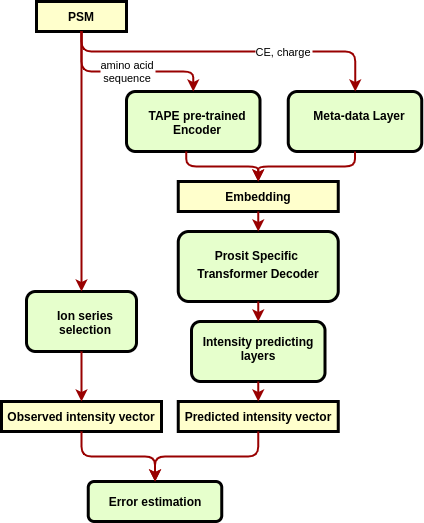
\includegraphics[width=6cm]{./img/architecture.png}
    \caption{{\bf The architecture of the Prosit Transformer.} The model depends on a pre-trained encoder from the TAPE project and uses the TAPE design for a Prosit Specific decoder. However, our model implements many of the design features of Prosit RNN, i.e., layers handling meta-data and final intensity prediction. \label{fig:architecture}}
\end{figure}
    

We set out to use the setup previously used for training and testing the Prosit model but with a transformer. We used the pre-trained TAPE model \cite{Rao2019-qq} and retrofitted it with a Prosit-specific decoder and some additional application-specific code (See Figure \ref{fig:architecture}). The TAPE model will encode the peptide into a 512-dimensional embedding. Furthermore, just as for the original RNN-based Prosit model, we used layers for handling meta-data consisting of the charge state of the spectrum and its collision energy (CE). The charge states range from one to six, represented as 6-dimensional one-hot-encoding. Hence, the meta-data layer has seven input nodes to account for the charge state and CE. The meta-layer transforms the metadata into a 512-dimensional vector that is subsequently is combined with the encoded peptide by element-wise multiplication. Then a Prosit-specific Transformer will decode this combined embedding. Lastly, a two-layered Multilayer perception (MLP) follows the decoding layer, serving as a prediction layer to predict the spectrum intensity. The MLP used activation by a hinge loss function constrained between 0 and 6 (a $\textit{RELU6}$ function) to activate the two final layers to avoid a so-called gradient explosion. For the training, the objective function was to minimize the sum of the angular distances between the observed and predicted spectrum intensity vectors.


\begin{figure}[htb!]
    \centering
    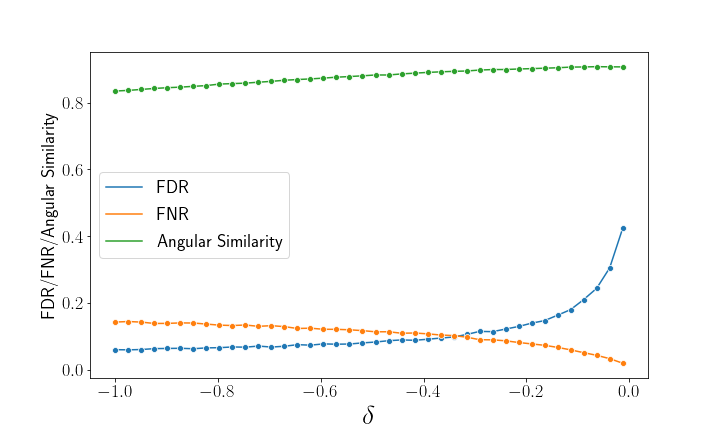
\includegraphics[width=8cm]{./img/compare_delta.png}
    \caption{{\bf The effect of adjusting the hyperparameter $\delta$ on predicting the absence/presence of individual MS2 peaks.} To obtain better prediction accuracy of present and absent MS2 peaks, we adjusted the intensities of absent peaks from zero to $\delta$. We measured the false discovery rate ($\mathit{FDR}$) and the false-negative rate ($\mathit{FNR}$) of each spectrum and then plotted the average angular similarity, the $\mathit{FDR}$, and the $\mathit{FNR}$ for different choices of $\delta$. We selected $\delta=0.34$ for the final training.  The predicted spectra were not post-processed for the measurements in this figure (See Methods). \label{fig:delta}}
\end{figure}
    
\subsection*{Training of model}

During the training, we used a batch size of 1024, the learning rate of 0.0001, gradient accumulation step of one, and a linear learning rate schedular with 10000 warmup steps. The training proceeded until no further improvement over ten epochs.

To better predict present and absent peaks, we introduced a hyperparameter, $\delta$, setting an artificial offset of the intensities of absent peaks to $\delta_p =\delta / |\rm{number\ of\ considered\ peaks}|$. This hyperparameter adds an extra penalty if the model predicts intensities for absent peaks. By varying the size of $\delta$, we can control the model’s propensity to predict peaks as absent, and by such means, tune the model’s false positive and false negative predictions. We measured the false discovery rate and the false-negative rate of each spectrum and then plotted the average angular similarity, the $\mathit{FDR}$, and the $\mathit{FNR}$ for different choices of $\delta$. We selected $\delta=0.34$ for the final training. (See Figure \ref{fig:delta})



\begin{figure}[tbh!]
    \centering
    \begin{tabular}{cc}
    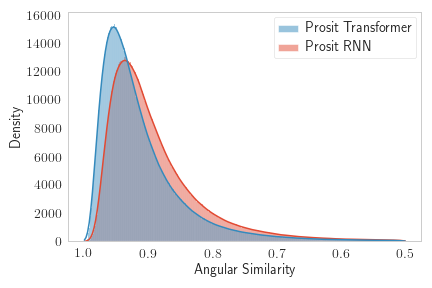
\includegraphics[width=6cm]{./img/spectralAngleDist.png} & 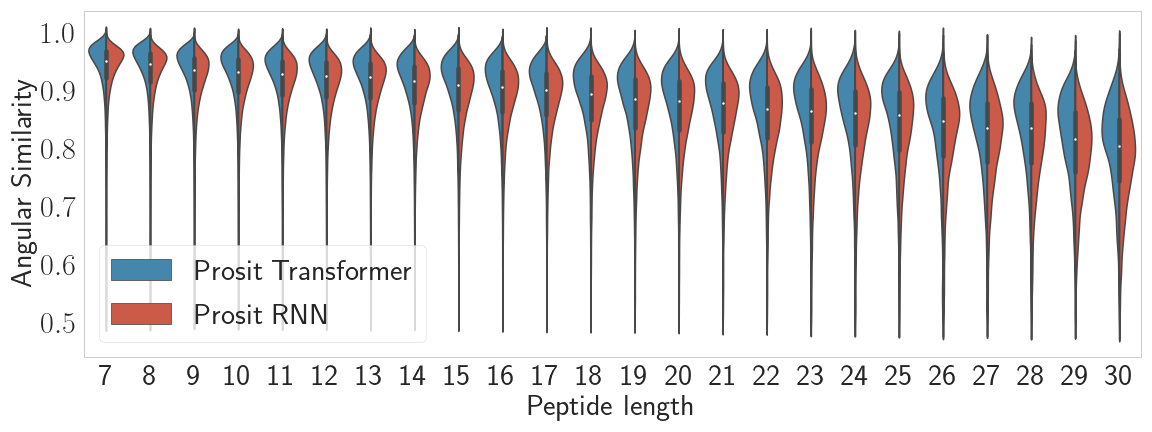
\includegraphics[width=8cm]{./img/violin_sa_pepLen.png}\\
    A & B \\
    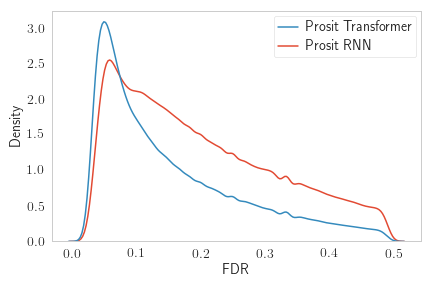
\includegraphics[width=6cm]{./img/fdr.png} & 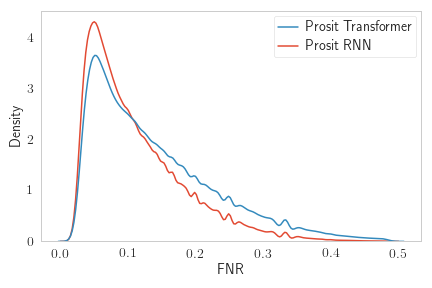
\includegraphics[width=6cm]{./img/fnr.png} \\
    C & D
    \end{tabular}
    \caption{{\bf Comparison of the accuracy of Prosit Transformer and Prosit RNN.} (A) We made separate histograms and smoothed them with a kernel density estimator to observe the distribution of angular similarity for the spectra predicted with Prosit Transformer and Prosit RNN. (B) The same angular similarity was also stratified by the length of peptides. (C) We also measured the false discovery rate, i.e., the fraction of observed absent peaks among the predicted non-zero intensity peaks for each spectrum, and (D) the false-negative rate, i.e., the fraction of predicted absent peaks among the observed non-zero intensity peaks.\label{fig:performance}}
    \end{figure}


\subsection*{Comparison of performance to regular Prosit}
    

To test the performance of our final Prosit Transformer, we investigated its performance on the same held-out test set as used when initially training Prosit RNN. We calculated the so-called angular similarity between the predicted and observed intensities for both predictors. Overall, we see that the predictions from Prosit Transformer have a higher angular similarity than Prosit RNN and are hence more accurate (Figure \ref{fig:performance}A). The Prosit Transformer increased the median angular similarity from Prosit RNN’s 0.908 to 0.929. We also see that Prosit Transformer obtained a higher angular similarity than Prosit RNN in 75.7\% of the spectra, while the opposite was true in 24.3\% of the spectra. The same pattern was also true when dividing the PSMs based on their peptide’s lengths (Figure \ref{fig:performance}B). We also wanted to compare the predictors’ ability to predict present and absent (zero intensity) fragment peaks.  Our choice of hyperparameter delta for Prosit Transformer resulted in a lower fraction of observed absent peaks among the predicted non-zero intensity peaks (Figure \ref{fig:performance}C) while observing a higher fraction of predicted absent peaks among the observed non-zero intensity peaks (Figure \ref{fig:performance}D) for Prosit Transformer compared to Prosit RNN.




\subsection*{Comparison of a Transformer to an extended RNN for prediction of spectra}

We set out to eliminate other explanations for Prosit Transformer's elevated performance than the Transformers themselves. A notable difference between Prosit RNN and Prosit Transformer is their difference in size. Prosit RNN contains 3 million parameters, while Prosit Transformer contains 163 million parameters, which gives the Transformer an unfair advantage. Hence, we stacked long short-term memory layers to create RNN models of similar size to the ones of the Transformers. This extended RNN gave a median angular similarity of 0.892 compared to Prosit Transformer's 0.929. Further, Prosit Transformer also outperformed the extended RNNs encoder in combination with Prosit Transformer’s decoder (median angular similarity of 0.927), as well as Prosit Transformer's encoder in combination with Prosit RNN's decoder (median angular similarity of 0.915). See Table \ref{tab:architecture} for an overview of the permutations of encoder decode architectures and their sizes.

When training the RNN-models, the learning rate had to be decreased from 0.0001 to 0.00008 to get the model to learn. Everything else was the same as for the Transformer-Transformer model. We also had to switch the gated recurrent unit (GRU) of the Prosit RNN to an LSTM to use the TAPE framework, leading to minor differences between the Extended Prosit RNN and Prosit RNN. 

Surprisingly, the extended RNN-RNN model got worse results than regular Prosit. The decrease could be due to that increase from 3M to 178M parameters leading to overfitting, requiring more data to justify such a massive model for the type of architecture. However, a performance increase was observed in all cases when adding a Transformer to the architecture. The most significant increase in performance appeared when implementing the Transformer as a decoder, i.e., after the peptide has been encoded and combined with the meta-data, and not in the peptide's encoding, although this improves the results as well. 

\begin{table}[htbp]
    \caption{{\bf Extended RNN models' size and performance.} We trained and tested different permutations of expanded RNNs and Transformers of comparable size and compared their prediction accuracy.}
      \begin{tabular}{r@{-}l|cccccccl}
      \hline
      \multicolumn{2}{c|}{Architecture for} & Encoder & Encoder & Encoder & Decoder & Decoder & Decoder & Total & Median Angular \\
      Encoder   & Decoder    & size    & layers & units & size    & layers & units   & size  & similarity \\
      \hline
      Transformer & Transformer & 85M   & 12 & 768 & 64M   & 9 & 768 & 164M  & 0.929 \\
      RNN & RNN & 77M   & 5 & 1028 & 93M   & 5 & 2056 & 178M  & 0.892 \\
      Transformer & RNN & 64M  & 9 & 768 & 94M   & 10 & 768  & 172M  & 0.9156 \\
      RNN & Transformer & 53M   & 6 & 768 & 113M   & 6 & 768  & 173M  & 0.927 \\
      \hline
      \end{tabular}%
    \label{tab:architecture}%
  \end{table}%

\subsection*{Time comparision of sprectrum prediciton}

Both regular Prosit and Prosit Transformer were timed for predicting $1000$, $10000$, and $100000$ spectra to see how much the increased model complexity for Prosit Transformer affects prediction time; see table \ref{tab:predictionTime} below. Prosit Transformer requires roughly 40 times more time, so there is a clear trade-off for prediction accuracy and time requirements. 

\begin{table}[htbp]
    \caption{{\bf The larger Transformer model needs more time to predict spectra.} We measured the required time to predict spectra from peptides for both Prosit RNN and Prosit Transformer.}
      \begin{tabular}{l|lll}
      \hline
      Number of predicted spectra & 1k & 10k  & 100k \\
      \hline
      Prosit RNN & 0.05 s & 0.5 s  & 4.7 s \\
      Prosit Transformer & 2 s    & 18 s   & 180 s \\
      \hline
      \end{tabular}%
    \label{tab:predictionTime}%
  \end{table}%
  

\subsection*{Prosit Transformer’s ability to model collision energy}

\begin{figure}[ht!]
    \centering
    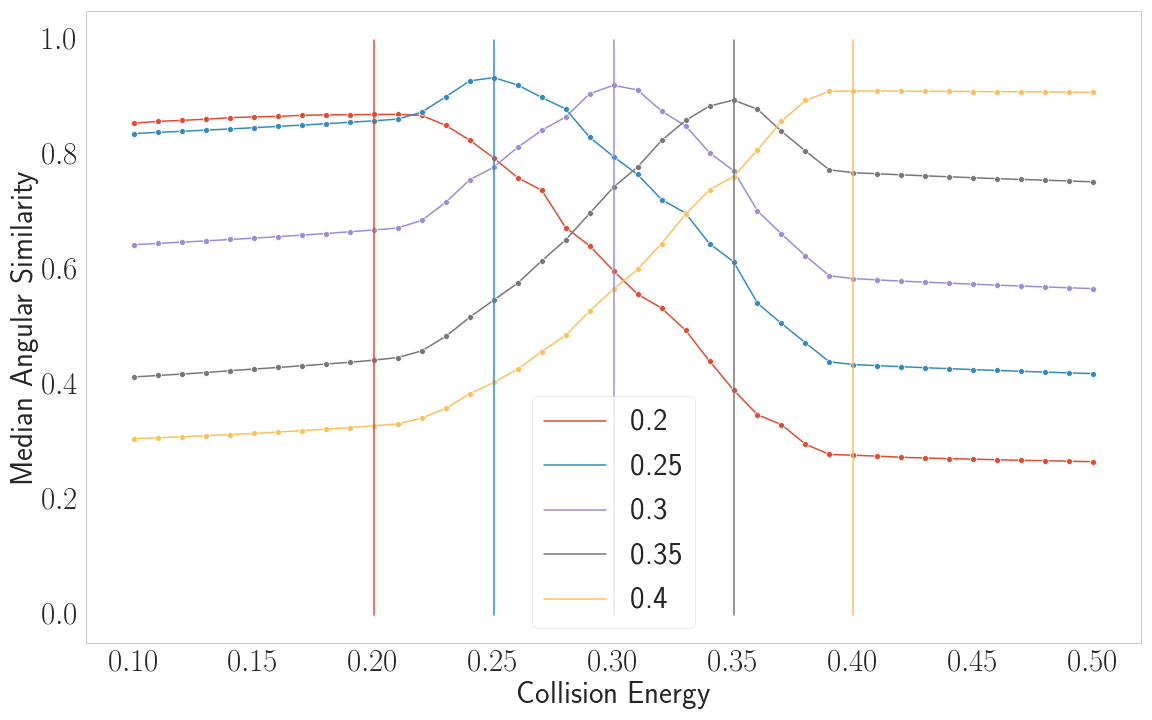
\includegraphics[width=12cm]{./img/ce_calibration.png}
    \caption{{\bf The mean spectral angle as a function of the collision energy (CE) for spectra acquired with different CEs.}\label{fig:ce}}
\end{figure}
    
We also wanted to test that the improved ability of Prosit Transformer to predict MS2 intensities did not affect the predictor’s ability to model collision energy’s (CE’s) influence on predicted spectra. We hence isolated batches of spectra with $\textit{CE}=\{0.2, 0.25, 0.3, 0.35, 0.4\}$ and measured the median Angular Similarity when predicting the spectra for a range of different collision energies (Figure \ref{fig:ce}). The highest angular similarity was found between the observed and predicted spectra when setting CE to the set’s actual specified value.

\section*{Discussion}
Here we have used a Transformer trained to predict protein sequence and transferred its functionality into predicting intensities of the b- and y- ions of MS2 spectra. The resulting predictor’s performance outperformed a predictor built by a classical recurrent neural network. This type of structure can likely improve other types of peptide property prediction.

One interesting finding was that the most significant improvement was when using Transformers as a decoder when comparing different combinations of RNNs and Transformers as decoders and encoders. A possible interpretation of this result is that Transformer architecture better utilizes the metadata, i.e., the collision energy and charge state information. A future direction of the project could be to investigate the source of the improved accuracy by examining the effects of removing this information from the different decoders.

Here we made use of the framework provided by the original Prosit project. It was essential to access the scripts and data sets provided and hardened by the previous team of algorithm designers. In general, it is of utmost importance to keep this type of resource easy to access. If we want to attract the attention of the machine learning community, which often wants a precise problem formulation and does not like to get into the details of how to generate datasets from scratch, we need to help them.


\section*{Acknowledgements}
Vital parts of this manuscript were conceived during the Dagstuhl Seminar 21271 on Computational Proteomics, July 2021.

The training of the Prosit Transformer model was enabled by the supercomputing resource Berzelius provided by National Supercomputer Centre at Linköping University and the Knut and Alice Wallenberg foundation.

\section*{Funding}

This work has been supported by a grant from the Swedish Foundation for Strategic Research (BD15-0043).

%\section*{Supporting information}

\bibliographystyle{unsrt}
\bibliography{transform}

\newpage
{\em For TOC Only:}\\[2em]
\centering
    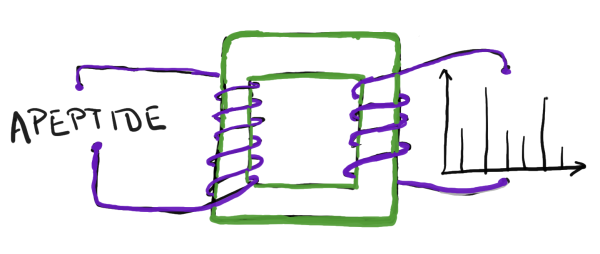
\includegraphics[width=10cm]{./img/transform.png}

\end{document}
